\definecolor{emerald}{RGB}{0, 168, 107}
\hypersetup{linkcolor=emerald}

\chapter{Test}
\label{chap:test}

\section{Test ``Analisi assistita''}
\noindent Per effettuare i test dell’estensione sono stati utilizzati alcuni siti realizzati per l’ultima edizione del concorso \textit{Accattivante Accessibile}.\
I test hanno preso in considerazione gli errori individuati da TV insieme a quelli segnalati dalla docente referente e sono stati messi a confronto con gli errori rilevati da \textit{SviluppAbile}.
Infine, ho confrontato i risultati elaborando un resoconto tabellare per ciascun sito analizzato e, successivamente, ho applicato la metrica F1-score per ottenere un report oggettivo.

\subsection{F1-score}
\noindent La F\textsubscript{1}-score è una metrica utilizzata per valutare modelli di classificazione, sia binari che multi‐classe. Essa combina in un unico valore la \textit{precision} (quanto le predizioni positive sono corrette) e il \textit{recall} (quanti casi positivi reali vengono identificati), calcolati come:

\[
\text{Precision} = \frac{TP}{TP + FP}, 
\qquad
\text{Recall} = \frac{TP}{TP + FN}
\]

\vspace{0.5cm}
\noindent L’F\textsubscript{1}-score è definita come la media armonica di tali valori:

\[
F_{1} = 2 \cdot \frac{\text{Precision} \cdot \text{Recall}}{\text{Precision} + \text{Recall}}
 = \frac{2 \cdot TP}{2 \cdot TP + FP + FN}
\]
\vspace{0.1cm}

\noindent Questo significa che nel calcolo verranno utilizzati i tre dati rilevati nel presente lavoro:
"errori trovati" come \(TP\) (veri positivi), "errori non trovati" come \(FN\) (falsi negativi), e \(FP\) (falsi positivi).
In questo modo, l’F\textsubscript{1}-score riflette in modo equilibrato sia la capacità di individuare correttamente errori reali, sia il controllo sui falsi allarmi.\\

\noindent L’F\textsubscript{1}-score assume valori compresi tra 0 e 1. Il valore minimo, \(0\), indica prestazioni pessime (almeno una delle due metriche è nulla), mentre il valore massimo, \(1\), corrisponde a prestazioni perfette (precisione e recall entrambi pari a 1).\\
Valori prossimi a 1 indicano quindi un buon funzionamento del sistema, mentre valori vicini a 0 segnalano performance insoddisfacenti.


% SUDOKU WORLD
\subsection{Sito web: SudokuWorld}
\noindent Di seguito vengono riportati alcuni dei test effettuati sul sito \href{https://caa.studenti.math.unipd.it/amonaco/Sudokuworld/pages/home.php}{SudokuWorld}.

\subsubsection{Total Validator}
\begin{figure}[H]
    \centering
    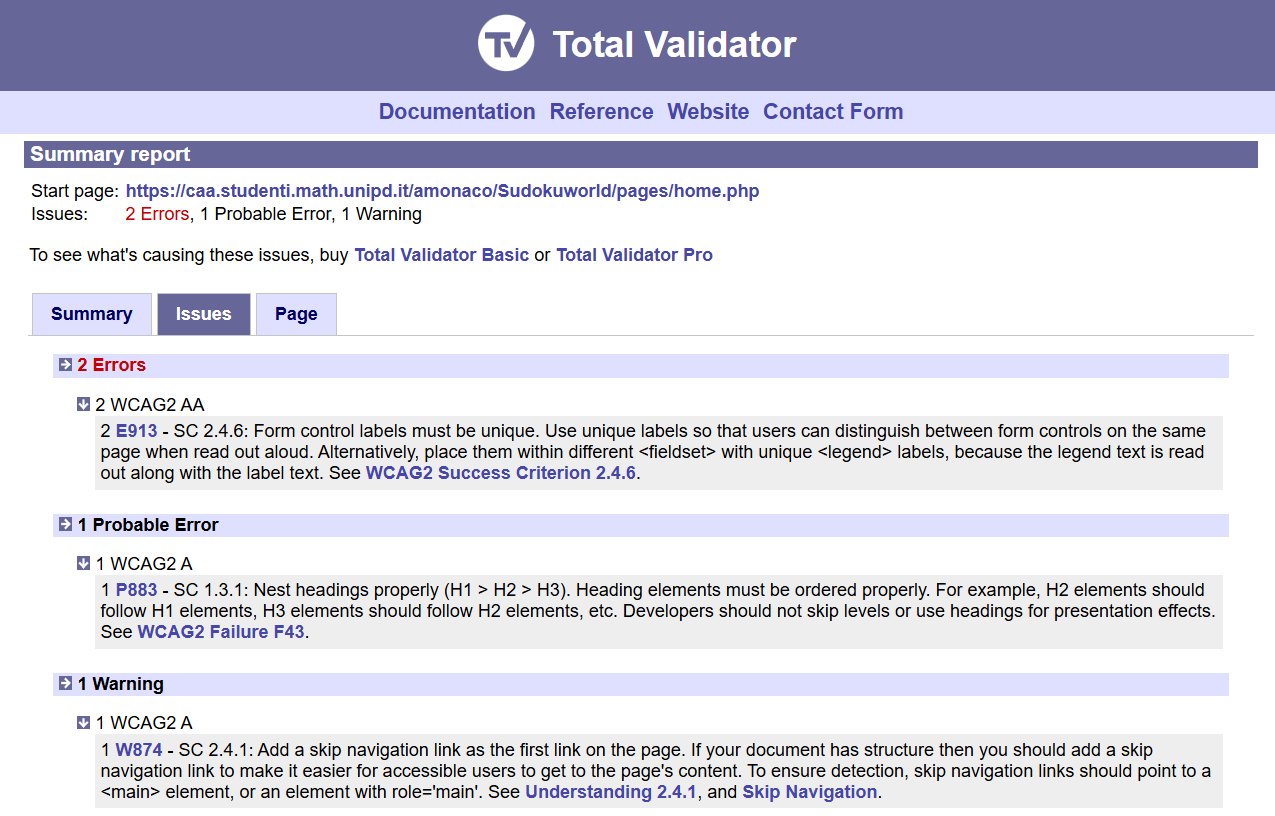
\includegraphics[width=0.7\linewidth, alt={Screenshot dell'analisi di Total Validator sul sito web SudokuWorld}]{img/TV_sudoku.png}
    \caption{Analisi di Total Validator sul sito web \textit{SudokuWorld}}\label{fig:TV_sudoku}
\end{figure}

\noindent L'analisi (vedi figura \ref{fig:TV_sudoku}) ha evidenziato due errori principali: etichette dei controlli dei form non univoche e intestazioni nidificate in modo non corretto. 
È stato inoltre segnalato un warning relativo all’assenza di un link di navigazione rapida. 
 
\subsubsection{Lighthouse}
\noindent Il report generato dallo strumento Lighthouse ha restituito un punteggio di 100/100 nella sezione Accessibility, indicando che, secondo le metriche automatiche adottate, non sono stati rilevati errori o problematiche di conformità (vedi figura \ref{fig:Lighthouse_sudoku}).
\begin{figure}[H]
    \centering
    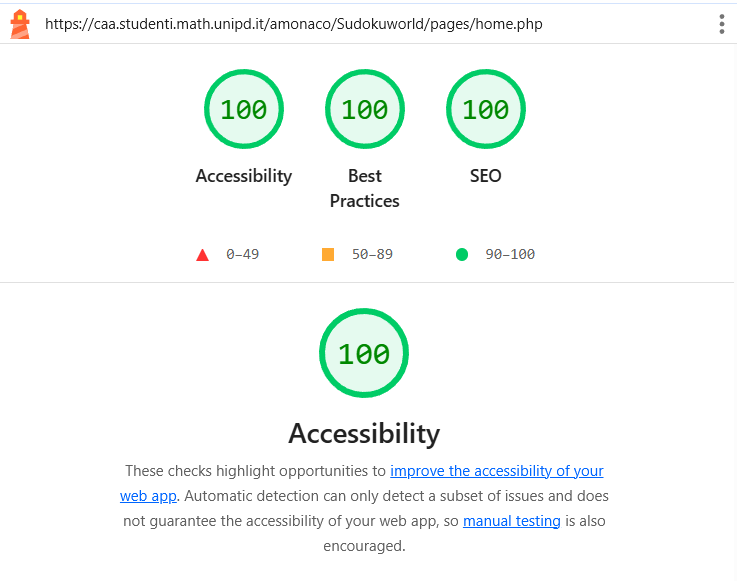
\includegraphics[width=0.6\linewidth, alt={Screenshot dell'analisi di Lighthouse sul sito web SudokuWorld}]{img/Lighthouse_sudoku.png}
    \caption{Analisi di Lighthouse sul sito web \textit{SudokuWorld}}\label{fig:Lighthouse_sudoku}
\end{figure}

\subsubsection{SviluppAbile}
\noindent Di seguito vengono riportati alcuni esempi di domande poste all’estensione \textit{SviluppAbile} e delle relative risposte ricevute. \newline
\\ \vspace{-0.5cm}
\noindent(pagina home.php)\\
\subsubsection*{\texttt{Il mio codice HTML rispetta le linee guida WCAG?}}
\begin{adjustwidth}{1cm}{1cm}
\noindent {\footnotesize Il tuo codice HTML sembra essere in parte conforme alle linee guida WCAG (Web Content Accessibility Guidelines), ma potrebbe migliorare ulteriormente per garantire una maggiore accessibilità. Alcune aree che richiedono ulteriore attenzione includono:\\
- L'attributo `aria-label` non è utilizzato in modo coerente nei controlli di navigazione.\\
- Le etichette dei pulsanti "Cerca" e "Profilo" potrebbero essere più descrittive.\\
Tuttavia, il tuo codice include molti elementi positivi come l'utilizzo di `alt` per immagini, la presenza di un titolo (`<title>`) e di metatag di descrizione (`<meta name="description">`). Questi sono passaggi fondamentali per migliorare la comprensione del contenuto da parte dei motori di ricerca e degli assistenti.\\
Per garantire una maggiore accessibilità, considera di applicare ulteriormente le linee guida WCAG 2.1, che offrono standard e raccomandazioni per creare esperienze web più inclusive.\\
La pagina non rispetta la norma W3C WCAG 2.1 che richiede di nidificare correttamente le intestazioni. Non sono presenti elementi HTML con attributo "h1", mentre ci sono intestazioni con grado inferiore.\\
La situazione descritta viola la regola WCAG 1.3.1, che richiede la corretta gerarchia di intestazioni (H1 > H2 > H3). In questo caso, l'h2 non è diretto al figlio dell'H1.\\
Vi è inoltre la presenza di due etichette (label) con il valore "Cerca" all'interno della stessa pagina HTML, ma con attributi id diversi ("searched-product" e "for"). Secondo la specifica SC 2.4.6, le etichette dei form control devono essere uniche.
}
\end{adjustwidth}

\subsubsection*{\texttt{Vi sono errori riguardanti i link?}}
\begin{adjustwidth}{1cm}{1cm}
\noindent {\footnotesize Il codice HTML contiene due carousel circolari:\\
1.  Il primo è definito come "specialProductsCarousel" e si trova nella sezione `<main>`.\\
2.  Il secondo è chiamato "bestSellersCarousel" ed è anch'esso presente all'interno della stessa sezione.\\
Quanto ai controlli sui link visitati, non sono implementati controlli specifici per la traccia dei link visitati sul sito web.
} \\
\end{adjustwidth}

\noindent(pagina sudoku.php)
\vspace{-0.5cm}
\subsubsection*{\texttt{Il mio codice HTML rispetta le linee guida WCAG?}} 
\begin{adjustwidth}{1cm}{1cm}
\noindent {\footnotesize Il tuo codice HTML non rispetta pienamente le linee guida WCAG (Web Content Accessibility Guidelines) per diverse ragioni:\\
1.  **La navigazione è troppo complessa**: la barra di navigazione contiene molti elementi e link, potrebbe essere difficile per gli utenti disabili utilizzare l'interfaccia.\\
2.  **L'accessibilità dei form è insufficiente**: non sono presenti attributi accessibili per i campi di input e submit, rendendo la navigazione dei form difficoltosa per gli utenti che usano dispositivi di assistenza.\\
3.  **La lettura dei testi in basso risulta difficile**: alcuni elementi come il timer sono troppo piccoli per essere letti facilmente dagli schermi con alto contrasto o da dispositivi di assistenza.\\
4.  **Non ci sono alternative al linguaggio naturale**: le immagini contengono solo icone e simboli, che potrebbero non essere compresi da utenti analfabetici.\\
\\Aggiungere attributi accessibili ai campi input e submit:\\
*   Modifica il codice HTML come segue:\\
    \texttt{<form class="d-flex align-items-center my-2 my-lg-0 ms-auto" \\ action="/amonaco/Sudokuworld/pages/search.php" method="GET"> 
    \begin{adjustwidth}{1cm}{}  <label for="searched-product" class="visually-hidden">Cerca</label>\end{adjustwidth}
    \begin{adjustwidth}{1cm}{} 
        <input class="form-control me-2" type="search" name="searched-product" id="searched-product" placeholder="Cerca" value="" aria-label="Search" />
    \end{adjustwidth}
    \begin{adjustwidth}{1cm}{} 
        <button class="btn btn-outline-success" type="submit" \textbf{aria-label="Submit the form"}>Cerca</button>
    \end{adjustwidth}
    </form>}\\
\\Aggiungere tag alt alle immagini: assicurati di aggiungere il contenuto alternativo per ogni immagine.\\
*   Modifica il codice HTML come segue:\\
    \texttt{<a class="nav-link" href="/amonaco/Sudokuworld/pages/sudoku.php">\\
    \indent <i class="bi bi-grid-3x3-gap-fill"></i>\\
    </a>}\\
\\Aggiungere tag aria: per fornire informazioni aggiuntive alle pagine web, puoi utilizzare gli attributi aria.\\
*   Modifica il codice HTML come segue:\\
    \texttt{<h1 class="container border border-black p-2 mb-4 rounded text-center" id="sudokuTitle" role="heading" aria-level="1">!! Sudoku !!</h1>}\\
\\Controlla l'accessibilità con strumenti di testing: prima della pubblicazione, assicurati di utilizzare strumenti come Lighthouse o WAVE per valutare la tua pagina web e risolvere eventuali problemi.\\
Ricorda che un sito web accessibile è più facile da utilizzare per tutti gli utenti, compresi quelli con disabilità.\\
\\
\texttt{DOMANDE SUGGERITE: \\"Quale è il criterio WCAG 2.1 che riguarda la navigazione con tastiera?"
\\"Come posso utilizzare gli strumenti di analisi del codice per identificare le aree dell'accessibilità da migliorare nel mio sito web HTML?"
}}
\end{adjustwidth}

\paragraph*{\texttt{"Come posso utilizzare gli strumenti di analisi del codice per \\ identificare le aree dell'accessibilità da migliorare nel mio sito web HTML?"}} 
\begin{adjustwidth}{1cm}{1cm}
\noindent {\footnotesize Per identificare le aree dell'accessibilità da migliorare nel tuo sito web HTML, puoi utilizzare gli strumenti di analisi come W3C Validator e Lighthouse. Il W3C Validator verifica la correttezza del codice HTML e fornisce suggerimenti per migliorare l'accessibilità. Lighthouse è uno strumento open-source che valuta l'accessibilità, le prestazioni e la sicurezza del tuo sito web.}
\end{adjustwidth}

\vspace{0.8cm}

\noindent \textbf{Resoconto finale dei test}\\
\noindent Di seguito viene illustrato il processo di test effettuato da \textit{SviluppAbile} confrontando i risultati ottenuti dagli altri strumenti di validazione e integrando anche un controllo manuale basato sulle Web Content Accessibility Guidelines (WCAG 2.1). Lo studio è stato articolato sulle principali pagine del sito, inclusa l’area riservata.\\

\noindent \textbf{Pagina home.php}\\
L’estensione \textit{SviluppAbile} ha rilevato la mancanza di una gerarchia corretta delle intestazioni: non è presente un elemento <h1>, mentre compaiono direttamente intestazioni di livello inferiore. Questo comportamento viola il criterio {\hyperref[wcag:1.3.1]{\textit{1.3.1 - Info and Relationships}}}, che prescrive una corretta nidificazione semantica. Inoltre, sono state individuate etichette duplicate per i campi di ricerca, contrarie al criterio {\hyperref[wcag:2.4.6]{\textit{2.4.6 - Headings and Labels}}}, ed un utilizzo incoerente di aria-label nei controlli di navigazione, che può generare confusione negli screenreader.
L’analisi manuale ha permesso di osservare ulteriori criticità, tra cui la mancanza di un meccanismo di bypass (skip link) in violazione del criterio {\hyperref[wcag:2.4.1]{\textit{2.4.1 - Bypass Blocks}}}, e l’assenza di landmark semantici <main> e <nav>.\\

\noindent \textbf{Pagina sudoku.php}\\
In questa pagina è stato rilevato che i form risultano privi di etichette accessibili e che i pulsanti non sono sufficientemente descrittivi, in contrasto con i criteri {\hyperref[wcag:3.3.2]{\textit{3.3.2 - Labels or Instructions}}} e {\hyperref[wcag:4.1.2]{\textit{4.1.2 - Name, Role, Value}}}. È stata inoltre segnalata l’assenza di testi alternativi per le icone, che viola il criterio {\hyperref[wcag:1.1.1]{\textit{1.1.1 - Non-text Content}}}. Alcuni elementi testuali, come il timer, presentano dimensioni ridotte e difficilmente leggibili, con possibili ricadute sul criterio {\hyperref[wcag:1.4.4]{\textit{1.4.4 - Resize Text}}}.
Un’osservazione manuale ha evidenziato che i contrasti cromatici non sempre soddisfano il rapporto minimo richiesto dal criterio {\hyperref[wcag:1.4.3]{\textit{1.4.3 - Contrast (Minimum)}}} e che non è garantita la piena navigabilità da tastiera ({\hyperref[wcag:2.1.1]{\textit{2.1.1}}}).\\

\noindent \textbf{Pagina search.php}\\
La pagina di ricerca consente agli utenti di filtrare e visualizzare i prodotti disponibili. 
L’estensione \textit{SviluppAbile} ha rilevato alcune criticità principali: assenza di intestazione <h1>, che viola il criterio {\hyperref[wcag:1.3.1]{\textit{1.3.1}}}, etichette duplicate nei campi di ricerca ({\hyperref[wcag:2.4.6]{\textit{2.4.6}}}) e uso incoerente di aria-label nei controlli di navigazione. Inoltre, il contrasto di alcuni elementi testuali non soddisfa il rapporto minimo previsto ({\hyperref[wcag:1.4.3]{\textit{1.4.3}}}).\\
L’analisi manuale ha evidenziato ulteriori problematiche: mancata navigabilità completa da tastiera ({\hyperref[wcag:2.1.1]{\textit{2.1.1}}}), assenza di landmark semantici come <main> e <nav> e testi alternativi mancanti per le icone o immagini illustrative ({\hyperref[wcag:1.1.1]{\textit{1.1.1}}}).\\

\noindent \textbf{Pagine product.php?id=…}\\
Le schede prodotto, come quelle relative alla tazza “I love sudoku” e alla maglia “commit sudoku”, hanno mostrato ulteriori problematiche. \textit{SviluppAbile} ha rilevato la mancanza di testi alternativi per le immagini ({\hyperref[wcag:1.1.1]{\textit{1.1.1}}}), l’assenza di titoli significativi nei tag <title> ({\hyperref[wcag:2.4.2]{\textit{2.4.2 - Page Titled}}}) e l’utilizzo non semantico del markup per i prezzi scontati ({\hyperref[wcag:1.3.1]{\textit{1.3.1}}}). Sono stati inoltre segnalati link privi di indicazioni chiare di stato focus o visited ({\hyperref[wcag:2.4.7]{\textit{2.4.7 - Focus Visible}}}) e la mancanza di attributi ARIA utili a descrivere pulsanti generici come “Aggiungi al carrello” ({\hyperref[wcag:4.1.2]{\textit{4.1.2}}}).
L’analisi manuale ha messo in luce ulteriori difetti: contrasti di colore insufficienti ({\hyperref[wcag:1.4.3]{\textit{1.4.3}}}), assenza di skip link ({\hyperref[wcag:2.4.1]{\textit{2.4.1}}}) e mancanza di landmark semantici ({\hyperref[wcag:1.3.1]{\textit{1.3.1}}}).\\

\noindent \textbf{Pagina carrello.php}\\
Sebbene l’estensione non abbia segnalato particolari criticità nella struttura della pagina, un’analisi manuale rivela che i prodotti nel carrello non sono accompagnati da testi alternativi adeguati per le immagini ({\hyperref[wcag:1.1.1]{\textit{1.1.1}}}), né da descrizioni sufficientemente univoche per i pulsanti di azione, come “Rimuovi” o “Procedi al pagamento”. La mancanza di etichette descrittive viola i criteri {\hyperref[wcag:2.4.6]{\textit{2.4.6}}} e {\hyperref[wcag:3.3.2]{\textit{3.3.2}}}. Inoltre, i controlli del carrello non garantiscono un chiaro stato di focus, contravvenendo al criterio {\hyperref[wcag:2.4.7]{\textit{2.4.7}}}.\\

\noindent \textbf{Pagina login.php}\\
L’accesso alla pagina di login con credenziali di test ha permesso di individuare alcune criticità: i campi di input risultano privi di etichette esplicite e i pulsanti sono generici, compromettendo la fruibilità per chi utilizza tecnologie assistive ({\hyperref[wcag:3.3.2]{\textit{3.3.2}}} e {\hyperref[wcag:4.1.2]{\textit{4.1.2}}}). Inoltre, non sono presenti attributi \texttt{aria-label} sui controlli di autenticazione.\\
L’analisi manuale ha messo in luce ulteriori problematiche non rilevate dallo strumento: la mancanza di messaggi di errore in caso di inserimento di credenziali errate ({\hyperref[wcag:3.3.1]{\textit{3.3.1 - Error Identification}}}), link come “Registrati” privi di testo descrittivo contestuale ({\hyperref[wcag:2.4.4]{\textit{2.4.4 - Link Purpose (In Context)}}}), e la mancanza di informazioni semantiche aggiuntive che faciliterebbero la navigazione da tastiera ({\hyperref[wcag:2.1.1]{\textit{2.1.1}}}). Queste osservazioni confermano che l’integrazione tra analisi automatica e verifica manuale è essenziale per una valutazione completa dell’accessibilità.\\

\noindent \textbf{Conclusioni}\\
Il confronto tra i risultati di SviluppAbile e l’analisi manuale basata sulle WCAG mostra come l’estensione sia efficace nell’individuare errori comuni e strutturali – quali la mancanza di testi alternativi, etichette duplicate, heading disordinati e pulsanti privi di descrizione – ma non riesca a rilevare altri aspetti fondamentali per l’accessibilità, come i contrasti cromatici, la presenza di skip link, la piena navigabilità da tastiera e l’utilizzo di landmark semantici.\\
Questo dimostra che uno strumento automatico, pur costituendo un valido supporto, deve ancora essere integrato con una verifica manuale alla luce delle linee guida ufficiali del W3C.

\paragraph{F1-score} \mbox{}\\
\noindent Nella tabella \ref{tab:sudokuWorld} vengono riassunti i risultati ottenuti.
\begin{footnotesize}
\begin{longtable}[c]{|C{4.8cm}|C{4.8cm}|C{4.8cm}|}
\caption{Tabella riassuntiva analisi \textit{SudokuWorld} tramite \textit{SviluppAbile}}
\label{tab:sudokuWorld}\\
\hline
\textbf{Errori trovati} & \textbf{Errori non trovati} & \textbf{Falsi positivi}\\
\hline
\endfirsthead
\multicolumn{3}{c}%
{{\bfseries Tabella \thetable\ -- continua dalla pagina precedente}} \\
\hline
\textbf{Errori trovati} & \textbf{Errori non trovati} & \textbf{Falsi positivi}\\
\hline
\endhead
\hline
\multicolumn{3}{r}{{ -- continua nella pagina successiva}} \\
\endfoot
\hline
\endlastfoot
\begin{itemize}
    \item h1 > h2 > h3
    \item Etichette dei form non univoche
    \item Errori con gli alt
    \item Errore button "registrati" 
    \item Link circolari
    \item Manca controllo link già visitati 
\end{itemize}
 & \begin{itemize}
    \item Contrasti dei colori
    \item Skip navigation link
\end{itemize}
 & \begin{itemize}
    \item Tag ARIA (suggerimenti errati)
    \item Suggerimenti alt errati
\end{itemize}\\
\hhline{|=|=|=|} 
6 & 2 & 2 \\
\end{longtable}
\end{footnotesize}

\noindent L'F\textsubscript{1}-score calcolato è $F_{1}=0.75$, un valore piuttosto buono che indica una capacità complessiva soddisfacente di individuare gli errori reali, pur con la presenza di alcuni mancati rilevamenti e di falsi positivi. 
Ciò suggerisce che l’estensione riesce a fornire risultati utili e affidabili, anche se rimane margine per ulteriori miglioramenti nella precisione e nella completezza dell’analisi.

% === DOLCE RISVEGLIO ===
\subsection{Sito web: Dolce Risveglio}
\noindent Di seguito vengono riportati alcuni dei test effettuati sul sito web \href{https://caa.studenti.math.unipd.it/gchecchi/}{Dolce Risveglio}.

\subsubsection{Total Validator}
\begin{figure}[H]
    \centering
    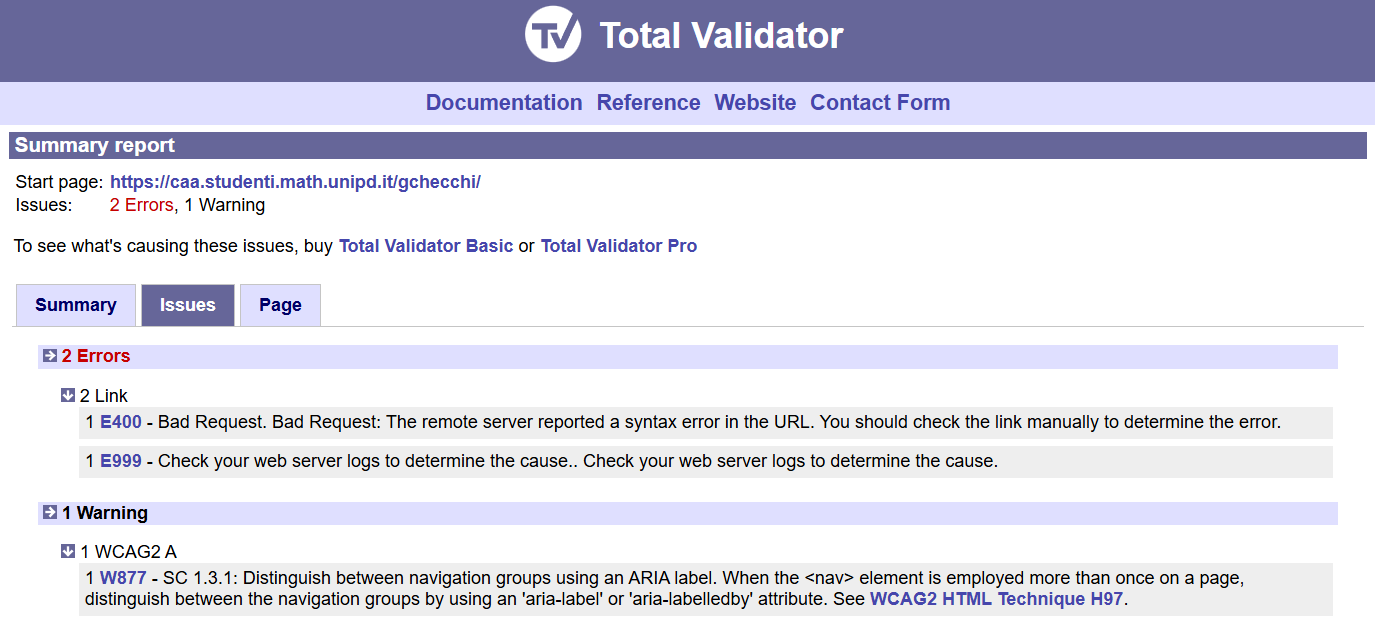
\includegraphics[width=0.9\linewidth, alt={Screenshot dell'analisi di Total Validator sul sito web Dolce Risveglio}]{img/TV_dolcerisveglio.png}
    \caption{Analisi di Total Validator sul sito web \textit{Dolce Risveglio}}\label{fig:TV_dolcerisveglio}
\end{figure}

\noindent L'analisi (vedi figura \ref{fig:TV_dolcerisveglio}) ha rilevato 2 errori relativi ai link e 1 warning. 
Gli errori comprendono un URL con richiesta non valida e un problema lato server da verificare nei log. 
Il warning riguarda la necessità di distinguere tra più aree di navigazione tramite un'etichetta ARIA. 

\subsubsection{Lighthouse}
\noindent Il report ha restituito un punteggio di 100/100 nella sezione \textit{Accessibility}, indicando che, secondo le metriche automatiche adottate, non sono stati rilevati errori o problematiche di conformità (vedi figura \ref{fig:Lighthouse_dolcerisveglio}).
\begin{figure}[H]
    \centering
    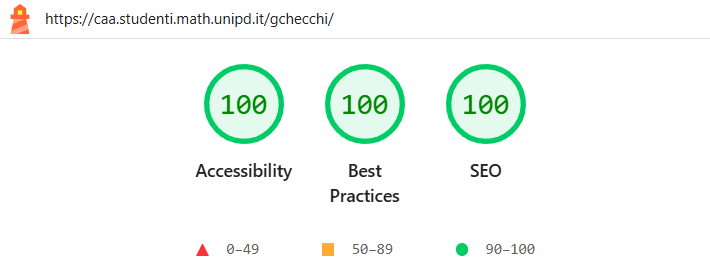
\includegraphics[width=0.6\linewidth, alt={Screenshot dell'analisi di Lighthouse sul sito web DolceRisveglio}]{img/Lighthouse_dolcerisveglio.png}
    \caption{Analisi di Lighthouse sul sito web \textit{Dolce Risveglio}}\label{fig:Lighthouse_dolcerisveglio}
\end{figure}

\subsubsection{Sviluppabile}
\noindent Di seguito viene illustrato il processo di test effettuato da \textit{SviluppAbile}, confrontando i risultati ottenuti dagli altri strumenti di validazione e integrando anche un controllo manuale basato sulle Web Content Accessibility Guidelines (WCAG 2.1). Lo studio è stato condotto sulle principali pagine del sito, inclusi i form di login, registrazione e le pagine informative.\\

\noindent \textbf{Pagina home.php}\\
La pagina \texttt{home.php} presenta una panoramica della caffetteria, con sezioni dedicate alla storia del locale, ai prodotti offerti e link al menù. L’estensione ha rilevato alcune criticità principali: immagini prive di testi alternativi ({\hyperref[wcag:1.1.1]{\textit{1.1.1 - Non-text Content}}}), uso di intestazioni senza gerarchia coerente ({\hyperref[wcag:1.3.1]{\textit{1.3.1 - Info and Relationships}}}) e suggerimenti per aggiungere label agli elementi interattivi eventualmente presenti nel footer ({\hyperref[wcag:2.4.6]{\textit{2.4.6 - Headings and Labels}}}).\\
L’analisi tramite strumenti automatici ha evidenziato ulteriori problemi: contrasto insufficiente in alcune aree di testo o link ({\hyperref[wcag:1.4.3]{\textit{1.4.3}}}), assenza di landmark semantici principali (\texttt{<main>} e \texttt{<nav>}) ({\hyperref[wcag:1.3.1]{1.3.1}}) e mancanza di skip link alternativi per navigare rapidamente al contenuto principale ({\hyperref[wcag:2.4.1]{\textit{2.4.1 - Bypass Blocks}}}).\\

\noindent \textbf{Pagina menu.php}\\
La pagina \texttt{menu.php} presenta il menù della caffetteria, con sezioni dedicate a bevande, pietanze e dolci, strutturate in liste e tabelle descrittive (\texttt{<dl>}). 
L’estensione \textit{SviluppAbile} ha rilevato alcune criticità principali: immagini dei piatti prive di testi alternativi significativi ({\hyperref[wcag:1.1.1]{1.1.1}}), bottoni per la selezione dei menu senza chiara indicazione dello stato attivo tramite attributi ARIA ({\hyperref[wcag:4.1.2]{\textit{4.1.2 - Name, Role, Value}}}) e suggerimenti per aggiungere label agli elementi interattivi ({\hyperref[wcag:2.4.6]{2.4.6}}).\\
Ulteriori controlli con strumenti automatici hanno evidenziato problemi come contrasti insufficienti tra testo e sfondo in alcune aree del menù ({\hyperref[wcag:1.4.3]{1.4.3}}) e assenza di skip link funzionanti per navigare rapidamente tra le sezioni del menù ({\hyperref[wcag:2.4.1]{2.4.1}}).\\

\noindent \textbf{Pagina contatti.php}\\
La pagina \texttt{contatti.php} consente agli utenti di inviare richieste o informazioni tramite un modulo di contatto, presentando campi per nome, email, telefono e messaggio. L’estensione ha rilevato alcune criticità principali: immagini prive di testi alternativi ({\hyperref[wcag:1.1.1]{1.1.1}}), campi del modulo senza indicazioni ARIA aggiuntive per facilitare la navigazione e la comprensione ({\hyperref[wcag:4.1.2]{4.1.2}}) e suggerimenti per aggiungere label più descrittive agli elementi interattivi presenti nel footer ({\hyperref[wcag:2.4.6]{2.4.6}}).\\
L’analisi tramite strumenti automatici ha evidenziato ulteriori problemi: contrasto insufficiente tra testo e sfondo in alcune aree ({\hyperref[wcag:1.4.3]{1.4.3}}), assenza di landmark semantici principali (\texttt{<main>} e \texttt{<nav>}) ({\hyperref[wcag:1.3.1]{1.3.1}}) e mancanza di skip link alternativi per navigare rapidamente al contenuto principale ({\hyperref[wcag:2.4.1]{2.4.1}}).\\

\noindent \textbf{Pagina prenotazioni.php}\\
La pagina \texttt{prenotazioni.php} permette agli utenti di prenotare un tavolo, specificando nome, email, telefono, giorno, orario e tavolo desiderato tramite un modulo strutturato. L’estensione ha rilevato alcune criticità principali: immagini prive di testi alternativi ({\hyperref[wcag:1.1.1]{1.1.1}}), campi del modulo senza indicazioni ARIA aggiuntive per facilitare la comprensione e l’interazione ({\hyperref[wcag:4.1.2]{4.1.2}}) e suggerimenti per aggiungere label più descrittive agli elementi interattivi presenti nel footer ({\hyperref[wcag:2.4.6]{2.4.6}}).\\
L’analisi tramite strumenti automatici ha evidenziato ulteriori problemi: contrasto insufficiente in alcune aree di testo ({\hyperref[wcag:1.4.3]{1.4.3}}), assenza di landmark semantici principali (\texttt{<main>} e \texttt{<nav>}) ({\hyperref[wcag:1.3.1]{1.3.1}}) e mancanza di skip link alternativi per navigare rapidamente al contenuto principale ({\hyperref[wcag:2.4.1]{2.4.1}}).\\

\noindent \textbf{Conclusioni}\\
Il confronto tra i risultati di \textit{SviluppAbile} e le verifiche effettuate con strumenti automatici mostra che l’estensione è efficace nell’individuare errori comuni di struttura e contenuto, come testi alternativi mancanti, etichette non descrittive e incongruenze tra attributi \texttt{required} e \texttt{aria-required}. Tuttavia, l’estensione non rileva completamente problematiche relative al contrasto cromatico, landmark semantici, skip link e piena navigabilità da tastiera.\\
Per ottenere una valutazione completa dell’accessibilità del sito, è necessario integrare l’uso di \textit{SviluppAbile} con controlli aggiuntivi basati sulle WCAG, assicurando che tutti i form abbiano label univoche, id coerenti e indicazioni ARIA appropriate.


\paragraph{F1-score} \mbox{}\\
\noindent Nella tabella \ref{tab:dolcerisveglio} vengono riportati i risultati ottenuti utilizzando l'estensione \textit{SviluppAbile}.
\begin{footnotesize}
\begin{longtable}[c]{|C{4.8cm}|C{4.8cm}|C{4.8cm}|}
\caption{Tabella riassuntiva analisi \textit{Dolce Risveglio} tramite \textit{SviluppAbile}}
\label{tab:dolcerisveglio}\\
\hline
\textbf{Errori trovati} & \textbf{Errori non trovati} & \textbf{Falsi positivi}\\
\hline
\endfirsthead
\multicolumn{3}{c}%
{{\bfseries Tabella \thetable\ -- continua dalla pagina precedente}} \\
\hline
\textbf{Errori trovati} & \textbf{Errori non trovati} & \textbf{Falsi positivi}\\
\hline
\endhead
\hline
\multicolumn{3}{r}{{ -- continua nella pagina successiva}} \\
\endfoot
\hline
\endlastfoot
\begin{itemize}
    \item Trovato solo da \textit{SviluppAbile}: alt non corretti delle img
    \item Etichette dei form non univoche
    \item Suggerisce l'aggiunta di label e id per gli elementi input
    \item Errore required e aria-required utilizzati insieme
\end{itemize}
 & 
\begin{itemize}
    \item Alcuni alt mancanti
\end{itemize}
 & \begin{itemize}
    \item Suggerisce un eccessivo uso di ARIA
\end{itemize}\\
\hhline{|=|=|=|} 
4 & 1 & 1 \\
\end{longtable}
\end{footnotesize}

\noindent L'F\textsubscript{1}-score calcolato è $F_{1}=0.8$, un risultato positivo che evidenzia una buona capacità di individuazione degli errori effettivi, con un numero limitato di falsi positivi e pochi elementi mancati.

% === E-LIXIRIUM ===
\subsection{Sito web: E-lixirium}
\noindent Di seguito vengono riportati alcuni dei test effettuati sul sito web \href{https://caa.studenti.math.unipd.it/abaldazz/?page=home}{E-lixirium}.
\subsubsection{Total Validator}
\begin{figure}[H]
    \centering
    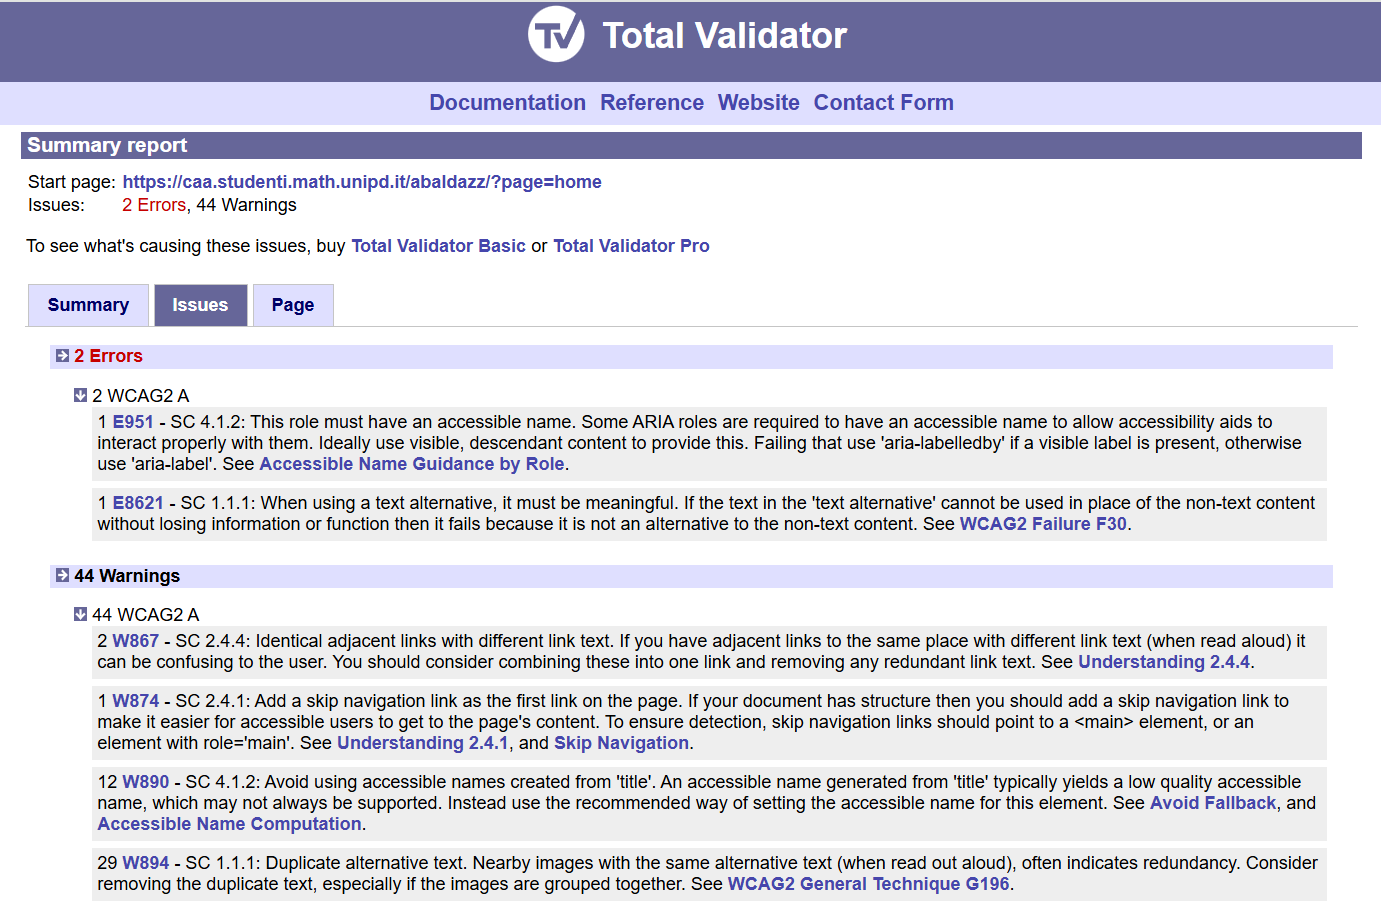
\includegraphics[width=0.8\linewidth, alt={Screenshot dell'analisi di Total Validator sul sito web E-lixirium}]{img/TV_elixirium.png}
    \caption{Analisi di Total Validator sul sito web \textit{E-lixirium}}\label{fig:TV_elixirium}
\end{figure}

\noindent L'analisi (vedi figura \ref{fig:TV_elixirium}) ha rilevato 2 errori principali e 44 warning. 
Gli errori riguardano principalmente elementi con ruoli ARIA a cui non è stato associato un nome accessibile e testi alternativi non significativi. Tra i warning, i più frequenti sono duplicazioni di testo alternativo per immagini, nomi accessibili generati da attributi \texttt{title}, link adiacenti con testi diversi e l’assenza di link di navigazione rapida. 

\subsubsection{Lighthouse}
\noindent Il report ha restituito un punteggio di 96/100 nella sezione \textit{Accessibility} (vedi figura \ref{fig:Lighthouse_elixirium}). 
Il problema segnalato riguarda il contrasto insufficiente tra colori di sfondo e primo piano, che può ridurre la leggibilità per alcuni utenti. 
\begin{figure}[H]
    \centering
    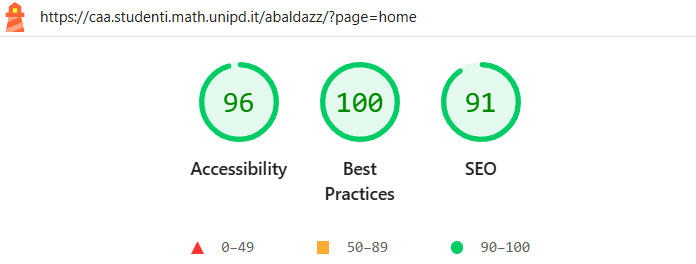
\includegraphics[width=0.6\linewidth, alt={Screenshot dell'analisi di Lighthouse sul sito web E-lixirium}]{img/Lighthouse_elixirium.png}
    \caption{Analisi di Lighthouse sul sito web \textit{E-lixirium}}\label{fig:Lighthouse_elixirium}
\end{figure}

\subsubsection{SviluppAbile}
\noindent \textbf{Pagina home}\\
La pagina \texttt{home} presenta la home page di \textit{E-lixirium}, con sezioni dedicate al logo, alla navigazione e alla presentazione di categorie e prodotti. L’estensione ha rilevato alcune criticità principali: immagini dei prodotti prive di testi alternativi significativi ({\hyperref[wcag:1.1.1]{\textit{1.1.1 - Non-text Content}}}), logo con link circolare verso la home anche quando l’utente è già sulla home ({\hyperref[wcag:2.4.4]{\textit{2.4.4 - Link Purpose (In Context)}}}), link adiacenti con testi diversi ma comportamento simile ({\hyperref[wcag:2.4.4]{2.4.4}}) e duplicazione di testi alternativi nelle stelle di valutazione dei prodotti ({\hyperref[wcag:1.1.1]{1.1.1}}).\\
L’analisi tramite strumenti automatici ha evidenziato ulteriori problemi: assenza di skip link per saltare la navigazione ({\hyperref[wcag:2.4.1]{\textit{2.4.1 - Bypass Blocks}}}), elementi della navbar nascosti tramite \texttt{display:none} invece di \texttt{visibility:hidden} ({\hyperref[wcag:2.1.1]{\textit{2.1.1 - Keyboard}}}), e link duplicati o circolari nella barra di navigazione ({\hyperref[wcag:2.4.4]{2.4.4}}).\\

\noindent \textbf{Pagina products}\\
La pagina \texttt{products} mostra l’elenco completo dei prodotti disponibili nel negozio E-lixirium. Come per la home page, si riscontrano criticità di accessibilità significative: le immagini dei prodotti utilizzano come testo alternativo il nome del file ({\hyperref[wcag:1.1.1]{1.1.1}}), le stelle di valutazione dei prodotti hanno alt duplicati o poco descrittivi ({\hyperref[wcag:1.1.1]{1.1.1}}), e non è presente uno skip link per saltare la navigazione ({\hyperref[wcag:2.4.1]{2.4.1}}).\\
Ulteriori problemi rilevati includono link duplicati o circolari nella barra di navigazione ({\hyperref[wcag:2.4.4]{2.4.4}}) e elementi nascosti tramite \texttt{display:none} invece di \texttt{visibility:hidden} ({\hyperref[wcag:2.1.1]{2.1.1}}). Alcuni link della navbar hanno testo identico ma conducono a destinazioni diverse ({\hyperref[wcag:2.4.4]{2.4.4}}), generando confusione per utenti con ausili assistivi.\\

\noindent \textbf{Pagina about}\\
La pagina \texttt{about} presenta informazioni sull’azienda E-lixirium e la sua missione, con testo descrittivo e un’immagine illustrativa. Dal punto di vista dell’accessibilità, si riscontrano le stesse criticità delle pagine precedenti: l’immagine ha un testo alternativo generico (\texttt{About E-lixirium}) che non descrive il contenuto visivo in dettaglio ({\hyperref[wcag:1.1.1]{1.1.1}}).\\
La struttura della pagina non prevede skip link per saltare la navigazione principale ({\hyperref[wcag:2.4.1]{2.4.1}}) e non tutti i link sono chiaramente descrittivi nel contesto ({\hyperref[wcag:2.4.4]{2.4.4}}). Inoltre, non vengono forniti attributi ARIA aggiuntivi per migliorare la fruibilità tramite lettori di schermo, e i pulsanti hanno colori e contrasto che potrebbero risultare insufficienti per utenti con difficoltà visive ({\hyperref[wcag:1.4.3]{\textit{1.4.3 - Contrast (Minimum)}}}).\\

\noindent \textbf{Conclusioni}\\
L’analisi complessiva delle tre pagine principali di \textit{E-lixirium} evidenzia una serie di criticità ricorrenti, in particolare relative ai testi alternativi delle immagini, alla gestione della navigazione e al contrasto visivo degli elementi interattivi. Le problematiche riscontrate potrebbero ostacolare l’accesso al sito da parte di utenti con disabilità visive o che utilizzano ausili tecnologici. Si consiglia di intervenire su testi alternativi più descrittivi, implementare skip link e migliorare il contrasto dei pulsanti e dei link, oltre a garantire una gestione coerente della navigazione e dei link duplicati, in linea con le linee guida WCAG 2.1.

\paragraph{F1-score} \mbox{}\\
\noindent Nella tabella \ref{tab:elixirium} vengono riportati i risultati ottenuti utilizzando l'estensione \textit{SviluppAbile}.
\begin{footnotesize}
\begin{longtable}[c]{|C{4.8cm}|C{4.8cm}|C{4.8cm}|}
\caption{Tabella riassuntiva analisi \textit{E-lixirium} tramite \textit{SviluppAbile}}
\label{tab:elixirium}\\
\hline
\textbf{Errori trovati} & \textbf{Errori non trovati} & \textbf{Falsi positivi}\\
\hline
\endfirsthead
\multicolumn{3}{c}%
{{\bfseries Tabella \thetable\ -- continua dalla pagina precedente}} \\
\hline
\textbf{Errori trovati} & \textbf{Errori non trovati} & \textbf{Falsi positivi}\\
\hline
\endhead
\hline
\multicolumn{3}{r}{{ -- continua nella pagina successiva}} \\
\endfoot
\hline
\endlastfoot
\begin{itemize}
    \item Errori di gestione della navigazione
    \item "display: none" da sostituire con "visibility: hidden"
    \item Link adiacenti identici con testi diversi
    \item Testo alternativo duplicato
\end{itemize}
 & 
\begin{itemize}
    \item Skip navigation link
    \item Link circolari nella navbar
    \item Logo con reindirizzamento nella home anche in home stesso
\end{itemize}
 & \\
\hhline{|=|=|=|} 
4 & 3 & 0 \\
\end{longtable}
\end{footnotesize}

\noindent L'F\textsubscript{1}-score calcolato è $F_{1}=0.73$, un risultato positivo che evidenzia come l’estensione abbia individuato correttamente la maggior parte degli errori presenti, pur lasciando tre problemi non rilevati. Non sono stati generati falsi positivi, il che indica un buon equilibrio tra precisione e completezza dell’analisi.


% === CORSA IDEALE ===
\subsection{Sito web: Corsa Ideale}
\noindent Di seguito vengono riportati alcuni dei test effettuati sul sito web \href{https://caa.studenti.math.unipd.it/epinarel/}{Corsa Ideale}.
\subsubsection{Total Validator}
\begin{figure}[H]
    \centering
    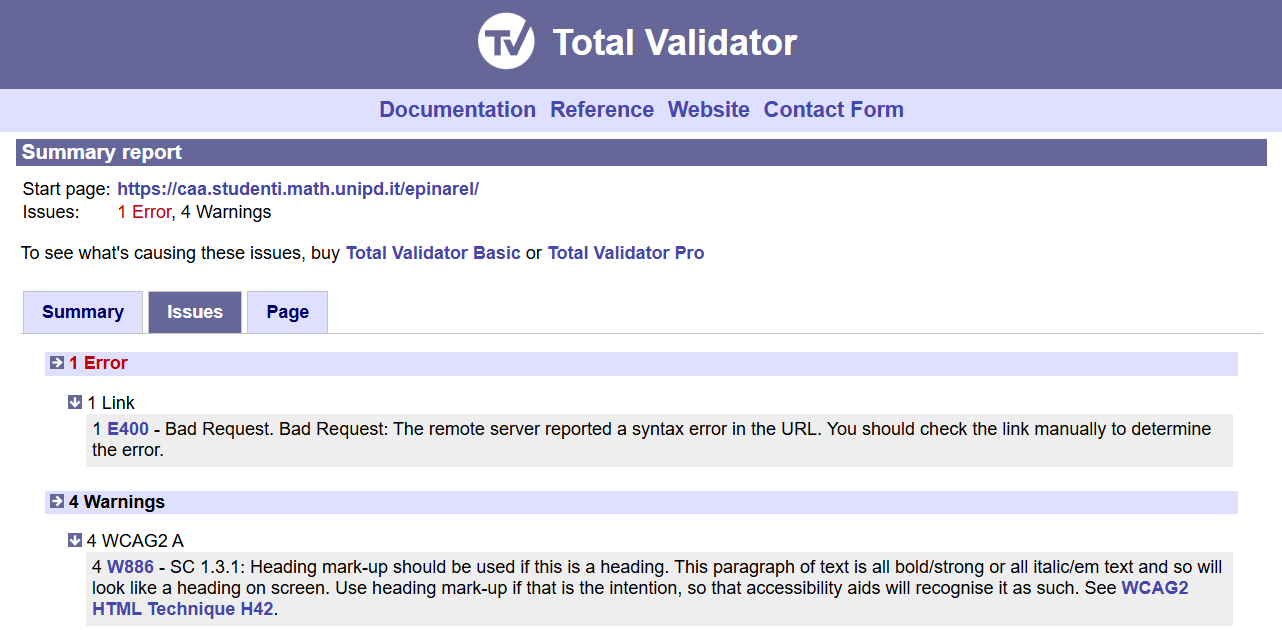
\includegraphics[width=0.8\linewidth, alt={Screenshot dell'analisi di Total Validator sul sito web Corsa Ideale}]{img/TV_corsaideale.png}
    \caption{Analisi di Total Validator sul sito web \textit{Corsa Ideale}}\label{fig:TV_corsaideale}
\end{figure}

\noindent \noindent L’analisi ha evidenziato un solo errore riguardante i link, dovuto a una richiesta non valida (\textit{Bad Request}), e quattro avvisi relativi all’uso improprio della marcatura tipografica (testi interamente in grassetto o corsivo che dovrebbero essere definiti come intestazioni). Questi warning non compromettono direttamente l’accessibilità, ma indicano buone pratiche di struttura da rispettare per garantire una corretta interpretazione da parte degli strumenti assistivi.

\subsubsection{Lighthouse}
\noindent Il report ha restituito un punteggio di 100/100 nella sezione \textit{Accessibility}, indicando che, secondo le metriche automatiche adottate, non sono stati rilevati errori o problematiche di accessibilità (vedi figura \ref{fig:Lighthouse_corsaideale}). 
Il problema segnalato riguarda il contrasto insufficiente tra colori di sfondo e primo piano, che può ridurre la leggibilità per alcuni utenti. 
\begin{figure}[H]
    \centering
    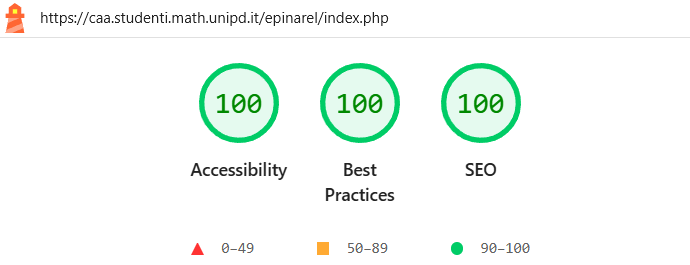
\includegraphics[width=0.6\linewidth, alt={Screenshot dell'analisi di Lighthouse sul sito web Corsa Ideale}]{img/Lighthouse_corsaideale.png}
    \caption{Analisi di Lighthouse sul sito web \textit{Corsa Ideale}}\label{fig:Lighthouse_corsaideale}
\end{figure}

\subsubsection{SviluppAbile}
\noindent \textbf{Pagina home}\\
La pagina \texttt{home} presenta il sito \texttt{CorsaIdeale}, con sezioni dedicate alla navigazione, alla presentazione delle ultime uscite, ai servizi offerti e ai ruoli dei corridori. Dal punto di vista dell’accessibilità, si riscontrano le seguenti criticità principali: immagini dei prodotti e del logo prive di testi alternativi significativi ({\hyperref[wcag:1.1.1]{\textit{1.1.1 - Non-text Content}}}), attributi \texttt{id} senza valore descrittivo o duplicati ({\hyperref[wcag:2.4.4]{\textit{2.4.4 - Link Purpose (In Context)}}}), etichette \texttt{label} non univoche ({\hyperref[wcag:3.3.2]{\textit{3.3.2 - Labels or Instructions}}}), chiusura di tag \texttt{p} erroneamente con \texttt{h3} ({\hyperref[wcag:1.3.1]{\textit{1.3.1 - Info and Relationships}}}) e nomi di attributi in maiuscolo anziché in minuscolo ({\hyperref[wcag:4.1.1]{\textit{4.1.1 - Parsing}}}).\\
La struttura della pagina prevede uno skip link per saltare la navigazione ({\hyperref[wcag:2.4.1]{2.4.1}}), ma non tutti i link della navbar sono chiaramente descrittivi nel contesto ({\hyperref[wcag:2.4.4]{2.4.4}}). Inoltre, non vengono utilizzati attributi ARIA aggiuntivi per migliorare la fruibilità tramite lettori di schermo, e alcune immagini decorative o informative non hanno alt appropriato ({\hyperref[wcag:1.1.1]{1.1.1}}).\\
Non sono stati riscontrati problemi relativi al contrasto dei colori ({\hyperref[wcag:1.4.3]{\textit{1.4.3 - Contrast (Minimum)}}}).\\

\noindent \textbf{Pagina lista.php}\\
La pagina \texttt{lista.php} mostra l’elenco delle scarpe con funzionalità di ricerca, filtro e ordinamento. 
L’estensione \textit{SviluppAbile} ha rilevato alcune criticità principali: assenza di testo alternativo significativo per le immagini delle scarpe e per il logo della navbar ({\hyperref[wcag:1.1.1]{1.1.1}}), utilizzo di \texttt{onclick} su interi blocchi cliccabili senza alternative da tastiera ({\hyperref[wcag:2.1.1]{\textit{2.1.1 - Keyboard}}}).\\
L’analisi tramite strumenti automatici ha evidenziato ulteriori problematiche: mancanza di landmark semantici coerenti come <main> e <nav> per ciascun blocco funzionale ({\hyperref[wcag:1.3.1]{1.3.1}}), etichette ridondanti o generiche nei pulsanti di filtro ({\hyperref[wcag:2.4.6]{\textit{2.4.6 - Headings and Labels}}}) e testi alternativi vuoti per le icone (menu, ricerca, like) ({\hyperref[wcag:1.1.1]{1.1.1}}).\\

\noindent \textbf{Pagina chi-siamo.php}\\
La pagina \texttt{chi-siamo.php} presenta informazioni sull’azienda, i valori e il team di CorsaIdeale. 
L’estensione ha rilevato alcune criticità principali: immagini senza testo alternativo significativo, compreso il logo e le foto dei membri del team ({\hyperref[wcag:1.1.1]{1.1.1}}), uso di \texttt{onclick} sui link del menu mobile senza alternative da tastiera ({\hyperref[wcag:2.1.1]{2.1.1}}).\\
L’analisi tramite strumenti automatici ha evidenziato ulteriori problematiche: mancanza di landmark semantici coerenti e completi per ciascun blocco di contenuto ({\hyperref[wcag:1.3.1]{1.3.1}}), etichette generiche o mancanti per alcuni link e pulsanti ({\hyperref[wcag:2.4.6]{2.4.6}}) e testi alternativi vuoti o poco descrittivi per le icone e immagini illustrative ({\hyperref[wcag:1.1.1]{1.1.1}}).\\

\noindent \textbf{Pagina accedi.php}\\
La pagina \texttt{accedi.php} consente agli utenti di autenticarsi e accedere alle funzionalità del sito CorsaIdeale. 
L’estensione \textit{SviluppAbile} ha rilevato alcune criticità principali: immagini del logo e del pulsante "torna su" prive di testo alternativo significativo ({\hyperref[wcag:1.1.1]{1.1.1}}), assenza di skip link per saltare direttamente al contenuto principale ({\hyperref[wcag:2.4.1]{2.4.1}}) e campi del form con placeholder utilizzati come unica indicazione ({\hyperref[wcag:2.4.6]{2.4.6}}).\\
L’analisi ha evidenziato ulteriori problemi: il form di login non è completamente fruibile tramite tastiera a causa di eventi \texttt{onblur} e \texttt{onclick} non sempre accessibili ({\hyperref[wcag:2.1.1]{2.1.1}}), la gestione dei messaggi di validazione non è semanticamente associata ai campi e alcuni link presentano testi generici ("Crea un nuovo account") senza indicare chiaramente la destinazione ({\hyperref[wcag:2.4.4]{2.4.4}}).\\

\noindent \textbf{Conclusioni}\\
L’analisi complessiva delle principali pagine di \textit{CorsaIdeale} evidenzia criticità ricorrenti, in particolare relative ai testi alternativi delle immagini, alla gestione della navigazione e all’accessibilità dei form e dei link. Le problematiche riscontrate potrebbero ostacolare l’accesso al sito da parte di utenti con disabilità visive o che utilizzano ausili tecnologici. Si consiglia di intervenire su testi alternativi più descrittivi, implementare skip link e garantire la fruibilità completa tramite tastiera, oltre a migliorare la gestione coerente della navigazione e dei link duplicati, in linea con le linee guida WCAG 2.1.

\paragraph{F1-score} \mbox{}\\
\noindent Nella tabella \ref{tab:corsaideale} vengono riportati i risultati ottenuti utilizzando l'estensione \textit{SviluppAbile}.
\begin{footnotesize}
\begin{longtable}[c]{|C{4.8cm}|C{4.8cm}|C{4.8cm}|}
\caption{Tabella riassuntiva analisi \textit{Corsa Ideale} tramite \textit{SviluppAbile}}
\label{tab:corsaideale}\\
\hline
\textbf{Errori trovati} & \textbf{Errori non trovati} & \textbf{Falsi positivi}\\
\hline
\endfirsthead
\multicolumn{3}{c}%
{{\bfseries Tabella \thetable\ -- continua dalla pagina precedente}} \\
\hline
\textbf{Errori trovati} & \textbf{Errori non trovati} & \textbf{Falsi positivi}\\
\hline
\endhead
\hline
\multicolumn{3}{r}{{ -- continua nella pagina successiva}} \\
\endfoot
\hline
\endlastfoot
\begin{itemize}
    \item Alt immagini vuoti
    \item Attributi id senza valore valido 
    \item Chiusura tag p erroneamente con tag h3 
    \item Label non univoca 
    \item Nomi attributi in maiuscolo anziché in minuscolo
\end{itemize}
 & \begin{itemize}
    \item Contrasto colori
\end{itemize}
 & \begin{itemize}
    \item Tag di heading usati in maniera scorretta
\end{itemize}\\
\hhline{|=|=|=|} 
5 & 1 & 1 \\
\end{longtable}
\end{footnotesize}

\noindent L'F\textsubscript{1}-score calcolato è $F_{1}=0.83$, un risultato positivo che evidenzia come l’estensione abbia rilevato correttamente la maggior parte degli errori presenti, lasciando un solo problema non individuato e generando un solo falso positivo.


% === BOOKOVERFLOW ===
\subsection{Sito web: BookOverflow}
\noindent Di seguito vengono riportati alcuni dei test effettuati sul sito \href{https://caa.studenti.math.unipd.it/lribon/}{BookOverflow}, sito web vincitore del concorso.
\subsubsection{Total Validator}
\begin{figure}[H]
    \centering
    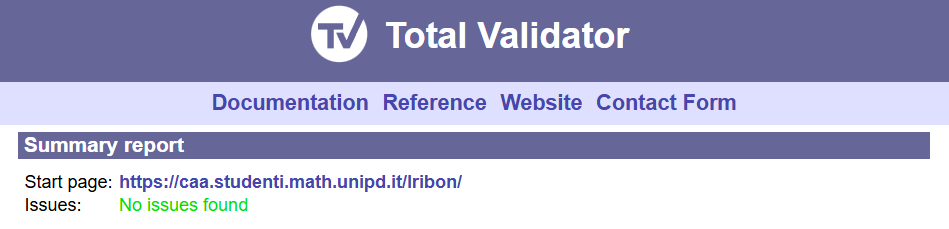
\includegraphics[width=0.8\linewidth, alt={Screenshot dell'analisi di Total Validator sul sito web BookOverflow}]{img/TV_bookoverflow.png}
    \caption{Analisi di Total Validator sul sito web \textit{BookOverflow}}\label{fig:TV_bookoverflow}
\end{figure}

\noindent Come visibile in figura \ref{fig:TV_bookoverflow}, non vi sono errori di accessibilità.

\subsubsection{Lighthouse}
\noindent Il report ha restituito un punteggio di 100/100 nella sezione \textit{Accessibility}, indicando che, secondo le metriche automatiche adottate, non sono stati rilevati errori o problematiche di accessibilità (vedi figura \ref{fig:Lighthouse_bookoverflow}).
\begin{figure}[H]
    \centering
    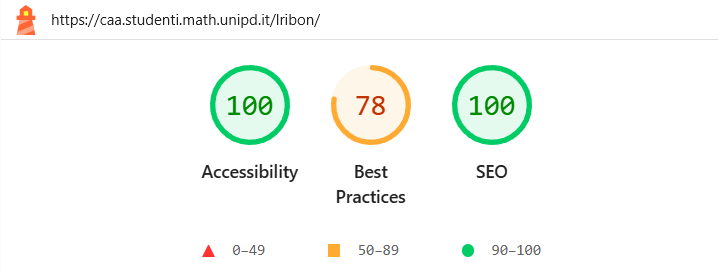
\includegraphics[width=0.6\linewidth, alt={Screenshot dell'analisi di Lighthouse sul sito web BookOverflow}]{img/Lighthouse_bookoverflow.png}
    \caption{Analisi di Lighthouse sul sito web \textit{BookOverflow}}\label{fig:Lighthouse_bookoverflow}
\end{figure}

\subsubsection{SviluppAbile}
\noindent \textbf{Pagina home.php}\\
La pagina \texttt{home.php} di BookOverflo introduce la piattaforma e mostra i libri più scambiati. 
L’estensione \textit{SviluppAbile} un uso inappropriato del tabindex sugli elementi interattivi ({\hyperref[wcag:2.1.1]{2.1.1}}).\\
L’analisi ha confermato invece che tutti gli elementi interattivi sono correttamente accessibili, l'analisi manuale invece si può notare che sembra non esservi un contrasto sufficiente tra link visitati e non visitati ({\hyperref[wcag:1.4.3]{1.4.3}}).

\noindent \textbf{Pagina esplora.php}\\
La pagina \texttt{esplora.php} consente agli utenti di scoprire nuovi libri, visualizzare i titoli più popolari e accedere a contenuti personalizzati dopo il login. 
L’estensione \textit{SviluppAbile} ha segnalato falsi positivi per uso inappropriato del tabindex sugli elementi interattivi ({\hyperref[wcag:2.1.1]{2.1.1}}).\\
L’analisi manuale ha confermato che tutti i link e i pulsanti sono etichettati in modo chiaro tramite attributi aria-label o testo visibilee tutte le immagini decorative o informative dispongono di testo alternativo appropriato ({\hyperref[wcag:1.1.1]{1.1.1}}, {\hyperref[wcag:1.3.1]{1.3.1}}, {\hyperref[wcag:2.4.6]{2.4.6}}). Inoltre, i contenuti personalizzati richiedono il login, ma i messaggi indicano chiaramente come accedere, senza compromettere l’accessibilità.\\

\noindent \textbf{Pagina come-funziona.php}\\
La pagina \texttt{come-funziona.php} illustra il funzionamento della piattaforma BookOverflow, spiegando agli utenti i vantaggi dello scambio libri e guidandoli passo passo attraverso la creazione della libreria, la selezione dei desideri e le modalità di spedizione. 
L’estensione \textit{SviluppAbile} non segnala alcun tipo di errore.

\noindent \textbf{Conclusioni}\\
In sintesi, la pagina risulta pienamente accessibile; le criticità segnalate da \textit{SviluppAbile} costituiscono falsi positivi dovuti alle ristrette capacità di analisi dell'IA alla base dell'estensione.\\


\paragraph{F1-score} \mbox{}\\
\noindent Nella tabella \ref{tab:bookoverflow} vengono riportati i risultati ottenuti utilizzando l'estensione \textit{SviluppAbile}.
\begin{footnotesize}
\begin{longtable}[c]{|C{4.8cm}|C{4.8cm}|C{4.8cm}|}
\caption{Tabella riassuntiva analisi \textit{BookOverflow} tramite \textit{SviluppAbile}}
\label{tab:bookoverflow}\\
\hline
\textbf{Errori trovati} & \textbf{Errori non trovati} & \textbf{Falsi positivi}\\
\hline
\endfirsthead
\multicolumn{3}{c}%
{{\bfseries Tabella \thetable\ -- continua dalla pagina precedente}} \\
\hline
\textbf{Errori trovati} & \textbf{Errori non trovati} & \textbf{Falsi positivi}\\
\hline
\endhead
\hline
\multicolumn{3}{r}{{ -- continua nella pagina successiva}} \\
\endfoot
\hline
\endlastfoot
 & 
\begin{itemize}
    \item Contrasto insufficiente link visitati/non
\end{itemize}
 & \begin{itemize}
    \item Tabindex non adeguato
\end{itemize}\\
\hhline{|=|=|=|} 
0 & 1 & 1 \\
\end{longtable}
\end{footnotesize}

\noindent L'F\textsubscript{1}-score calcolato è $F_{1}=0$, valore che indica prestazioni non soddisfacenti in questo caso specifico. 
Ciò evidenzia la necessità di ulteriori miglioramenti nell’identificazione degli errori, soprattutto per quanto riguarda i falsi positivi.

% === LUZZAUTO ===
\subsection{Sito web: LuzzAuto}
\noindent Di seguito vengono riportati alcuni dei test effettuati sul sito web \href{https://caa.studenti.math.unipd.it/eartusi/index.php}{LuzzAuto}.
\subsubsection{Total Validator}
\begin{figure}[H]
    \centering
    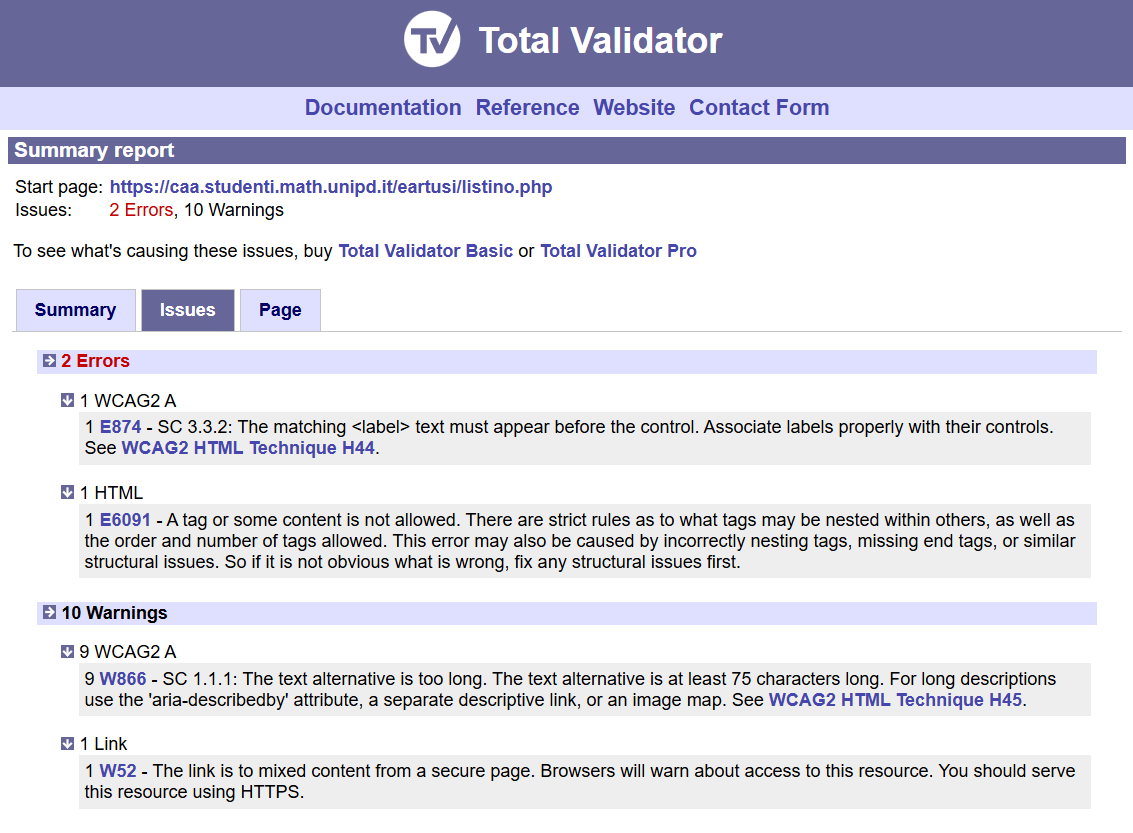
\includegraphics[width=0.8\linewidth, alt={Screenshot dell'analisi di Total Validator sul sito web LuzzAuto}]{img/TV_luzzauto.png}
    \caption{Analisi di Total Validator sul sito web \textit{LuzzAuto}}\label{fig:TV_luzzauto}
\end{figure}

\noindent Nella pagina \texttt{home.php} non sono presenti errori di accessibilità, ma solamente un "Warning" riguardante testi alternativi (\texttt{alt}) troppo lunghi. 
Nella pagina \texttt{listino.php} (come visibile in figura \ref{fig:TV_luzzauto}), sono segnalati due errori principali: 
uno relativo all'associazione corretta delle etichette ai rispettivi controlli e uno di struttura HTML, dovuto all'uso di tag non consentiti o a un errato annidamento degli stessi. 

\subsubsection{Lighthouse}
\noindent Il report ha restituito un punteggio di 100/100 nella sezione \textit{Accessibility}, indicando che, secondo le metriche automatiche adottate, non sono stati rilevati errori o problematiche di accessibilità (vedi figura \ref{fig:Lighthouse_luzzauto}).
\begin{figure}[H]
    \centering
    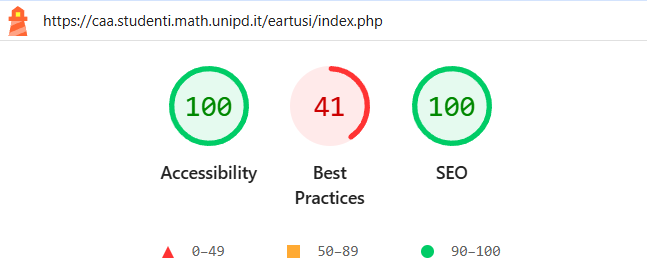
\includegraphics[width=0.6\linewidth, alt={Screenshot dell'analisi di Lighthouse sul sito web LuzzAuto}]{img/Lighthouse_luzzauto.png}
    \caption{Analisi di Lighthouse sul sito web \textit{LuzzAuto}}\label{fig:Lighthouse_luzzauto}
\end{figure}

\subsubsection{SviluppAbile}


\paragraph{F1-score} \mbox{}\\
\noindent Nella tabella \ref{tab:luzzauto} vengono riportati i risultati ottenuti utilizzando l'estensione \textit{SviluppAbile}.
\begin{footnotesize}
\begin{longtable}[c]{|C{4.8cm}|C{4.8cm}|C{4.8cm}|}
\caption{Tabella riassuntiva analisi \textit{LuzzAuto} tramite \textit{SviluppAbile}}
\label{tab:luzzauto}\\
\hline
\textbf{Errori trovati} & \textbf{Errori non trovati} & \textbf{Falsi positivi}\\
\hline
\endfirsthead
\multicolumn{3}{c}%
{{\bfseries Tabella \thetable\ -- continua dalla pagina precedente}} \\
\hline
\textbf{Errori trovati} & \textbf{Errori non trovati} & \textbf{Falsi positivi}\\
\hline
\endhead
\hline
\multicolumn{3}{r}{{ -- continua nella pagina successiva}} \\
\endfoot
\hline
\endlastfoot
\begin{itemize}
    \item Le etichette dei controlli non sono state associate correttamente ai rispettivi elementi.
\end{itemize} & 
\begin{itemize}
    \item Tag o contenuto non consentito. 
\end{itemize}
 & \\
\hhline{|=|=|=|} 
1 & 1 & 0 \\
\end{longtable}
\end{footnotesize}

\noindent L'F\textsubscript{1}-score calcolato è $F_{1} \approx 0.67$, un valore intermedio che evidenzia un discreto equilibrio tra errori rilevati e mancati. 
Pur non trattandosi di un risultato ottimale, esso mostra la capacità dell’estensione di individuare correttamente una parte significativa dei problemi, lasciando spazio a ulteriori miglioramenti.

\section{Test ``Modalità guidata''}
\noindent Per effettuare i test utili a dimostrare l'efficacia di \textit{SviluppAbile}, ho creato una semplice pagina \acrshort{html} (vedi figura \ref{fig:pagina_test}).
\begin{figure}[H]
    \centering
    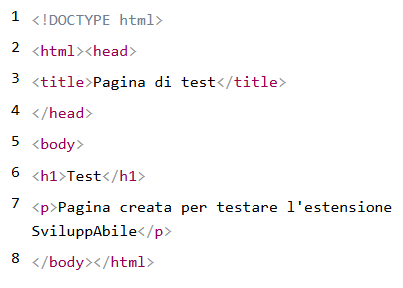
\includegraphics[width=0.5\linewidth, alt={Pagina \acrshort{html} base per effettuare i test della modalità guidata}]{img/test_MG.png}
    \caption{Pagina HTML base per effettuare i test della modalità guidata}\label{fig:pagina_test}
\end{figure}

\subsubsection*{\texttt{Come si crea un <head> che contenga tutti gli elementi utili per una pagina accessibile?}}
\begin{adjustwidth}{1cm}{1cm}
\noindent {\footnotesize Per creare un head accessibile, assicurati di includere i seguenti elementi:\\
1.  **Metatag Titolo (title)**: Utilizzato dal browser come titolo della finestra della pagina.\\
2.  **Metatag Descrizione (description)**: Descrive il contenuto della pagina e appare nella barra degli strumenti del browser e nei risultati dei motori di ricerca.\\
3.  **Metatag Chiave (keywords)**: Non più importante come in passato, ma puoi utilizzarla se necessario per le ricerche.\\
\\Inoltre, assicurati di utilizzare un markup semantico corretto per le sezioni della pagina. Ad esempio, puoi utilizzare `<header>`, `<nav>`, `<main>`, `<section>`, `<article>`, `footer>` in luogo di semplici div.\\
Infine, assicurati di aggiungere un elemento `alt` a tutte le immagini con una descrizione del contenuto dell'immagine.\\
\\CODICE SUGGERITO:\\
\texttt{1 <head>\\
2 <title>Pagina di test</title>\\
3 <meta charset="UTF-8">\\
4 <meta name="viewport" content="width=device-width, initial-scale=1.0">\\
5 <meta name="description" content="Pagina creata per testare l'estensione SviluppAbile">\\
6 <meta name="keywords" content="test,sviluppo accessibile">\\
7 </head>\\}}
\end{adjustwidth}


\subsubsection*{\texttt{Come posso ora creare dei paragrafi che rispettino le linee guida BEM?}}
\begin{adjustwidth}{1cm}{1cm}
\noindent {\footnotesize Per creare paragrafi in base alle linee guida BEM, puoi utilizzare la sintassi seguente:\\
1. Definisci un classico `.block\_\_element` per il contenuto del paragrafo: `class="block\_\_element"`\\
2. Utilizza `.block\_\_element--modificatore` per aggiungere modificatori: `class="block\_\_element --modificatore"`\\
In questo modo, i paragrafi saranno distinti e facili da identificare tramite la tecnica BEM.\\
\\Nota: Assicurati di sostituire `--modificatore` con il nome del modificatore effettivo nel tuo progetto.\\
\\CODICE SUGGERITO:\\
\texttt{1 <h1 class="block\_\_title">Titolo</h1>\\
2 <p class="block\_\_text --grande">Testo di esempio con un modificatore per il colore.</p>\\
3 <p class="block\_\_text --rosso">Testo di esempio con altro contenuto.</p>}\\
}
\end{adjustwidth}


\subsubsection*{\texttt{Come posso inserire immagini accessibili?}}
\begin{adjustwidth}{1cm}{1cm}
\noindent {\footnotesize Inserire immagini accessibili significa garantire che le informazioni contenute nelle immagini siano anche disponibili ai utenti con disabilità visiva. Ciò può essere fatto utilizzando l'attributo `alt` all'interno dell'elemento `<img>`.\\
In questo esempio, l'attributo `alt` contiene una descrizione breve e concisa della foto. Se il browser non è in grado di visualizzare l'immagine (ad esempio, se si utilizza un lettore schermo), la descrizione contenuta nell'attributo `alt` verrà visualizzata al posto dell'immagine.\\
Inoltre, per immagini decorative o grafici che non contengono informazioni importanti, è consigliabile utilizzare l'attributo `alt=""`, in modo da eliminare il testo alternativo dalla navigazione.\\
\\CODICE SUGGERITO:\\
\texttt{1 <img src="immagine.jpg" alt="Descrizione della foto">}
}
\end{adjustwidth}

\subsubsection*{\texttt{Come si crea una table rispettando le linee guida WCAG?}}
\begin{adjustwidth}{1cm}{1cm}
\noindent {\footnotesize Per creare una tabella accessibile secondo le linee guida WCAG, è importante fornire un'esperienza utente inclusiva e facilitare l'accessibilità a tutte le persone, in particolare alle persone con disabilità visive che utilizzano strumenti di lettura ad alta voce o tastiera. Ecco alcuni passaggi per creare una tabella accessibile:\\
1.  **Istruzioni per l'utilizzo della tabella**: fornire un'introduzione sulle informazioni presentate nella tabella e quali sono le colonne principali, aiutando gli utenti che utilizzano strumenti di lettura ad alta voce.\\
2.  **Tabella semantica con role="presentation" impostato su false**: questo ti permetterà a un assistente di lettura di comprendere il contenuto della tabella e fornirlo correttamente all'utente.\\
\\Nota che ogni elemento della tabella (celle, intestazioni) deve avere un id o un attributo aria-*, per fornire una descrizione dell'elemento e aiutare gli utenti con disabilità visive a comprendere il contenuto.\\
\\CODICE SUGGERITO:\\
\texttt{1 <table>\\
2 <caption>Esempio di tabella accessibile</caption>\\
3 <thead>\\
4 <tr role="row">\\
5 <th scope="col" id="nome">Nome</th>\\
6 <th scope="col" id="età">Età</th>\\
7 </tr>\\
8 </thead>\\
9 <tbody>\\
10 <tr role="row">\\
11 <td headers="nome">Mario Rossi</td>\\
12 <td headers="età">32 anni</td>\\
13 </tr>\\
14 <tr role="row">\\
15 <td headers="nome">Giovanni Bianchi</td>\\
16 <td headers="età">35 anni</td>\\
17 </tr>\\
18 </tbody>\\
19 </table>}
}
\end{adjustwidth}


\subsubsection*{\texttt{Come posso utilizzare gli attributi ARIA per migliorare l'accessibilità degli elementi interattivi?}}
\begin{adjustwidth}{1cm}{1cm}
\noindent {\footnotesize Gli attributi ARIA (Accessible Rich Internet Applications) sono stati sviluppati per rendere le applicazioni web accessibili a tutti, nonostante eventuali disabilità. Sono utilizzati per aggiungere funzionalità di navigazione e controllo agli elementi interattivi come i bottoni e gli elementi dropdown.\\
Per migliorare l'accessibilità degli elementi interattivi tramite ARIA, ti suggerisco di utilizzare le seguenti strategie:\\
1.  Utilizza il role di un elemento (ad esempio `button`, `menuitem`) per specificarne la funzione.\\
2.  Aggiungi gli attributi aria-label e aria-describedby per fornire una descrizione dell'elemento interattivo.\\
3.  Utilizza l'attributo aria-haspopup per indicare se un elemento è un menu o una lista.\\
\\In questo modo, l'elemento interattivo sarà più facile da navigare e controllare tramite strumenti assistivi come screen reader e mouse navigator.\\
Per ulteriori informazioni sugli attributi ARIA, ti consiglio di consultare la documentazione ufficiale dell'W3C.\\
\\CODICE SUGGERITO:\\
\texttt{1 <!DOCTYPE html>\\
2 <html><head>\\
3 <title>Pagina di test</title>\\
4 </head>\\
5 <body>\\
6 <!-- Utilizzo del role e degli attributi ARIA per il bottone -->\\
7 <button role="button" aria-label="Clicca per eseguire l'azione"> Esegui azione </button>\\
8 <!-- Utilizzo del role e degli attributi ARIA per il menu -->\\
9 <ul role="menu">\\
10 <li role="presentation">\\
11 <a href="\#" aria-label="Opzione 1" aria-haspopup="true">Opzione 1</a>\\
12 <ul role="sottomenu">\\
13 <li role="presentation"><a href="\#" aria-label="Sottopagina 1.1">Sottopagina 1.1</a></li>\\
14 <li role="presentation"><a href="\#" aria-label="Sottopagina 1.2">Sottopagina 1.2</a></li>\\
15 </ul></li></ul>\\
16 </body></html>}
}
\end{adjustwidth}

\section{Lista WCAG citate}
\begin{itemize}
    \item \label{wcag:1.1.1} 1.1.1 - Non-text Content
    \item \label{wcag:1.3.1} 1.3.1 - Info and Relationships
    \item \label{wcag:1.4.3} 1.4.3 - Contrast (Minimum)
    \item \label{wcag:1.4.4} 1.4.4 - Resize Text
    \item \label{wcag:2.1.1} 2.1.1 - Keyboard
    \item \label{wcag:2.4.1} 2.4.1 - Bypass Blocks
    \item \label{wcag:2.4.2} 2.4.2 - Page Titled
    \item \label{wcag:2.4.4} 2.4.4 - Link Purpose (In Context)
    \item \label{wcag:2.4.6} 2.4.6 - Headings and Labels
    \item \label{wcag:2.4.7} 2.4.7 - Focus Visible
    \item \label{wcag:2.4.8} 2.4.8 - Location
    \item \label{wcag:2.4.9} 2.4.9 - Link Purpose (Link Only)
    \item \label{wcag:3.3.1} 3.3.1 - Error Identification
    \item \label{wcag:3.3.2} 3.3.2 - Labels or Instructions
    \item \label{wcag:4.1.2} 4.1.2 - Name, Role, Value
\end{itemize}


